\section{Loss function}


\subsection{Commonly used loss functions in neural compression}
As with most other areas in deep learning, many different loss functions are prevalent in the field of neural lossy image compression. The mean squared error (MSE) is quite common\cite{benchmark} and has been used to get some quite good results \cite{endToend}. In many areas of machine learning, the MSE is a default choice because it helps closing the gap between between the prediction and the wanted result. However, when working with lossy image compression, the ultimate judge is going to be the people looking at the images! Thus it is evident that since the loss function influences what data is favoured by the model, the loss function needs to align well with the human visual system (HVS), in order for the model to generate great reconstructions of the original image\cite{msebad}\cite{SSIM}. Unfortunately the MSE does not align that well with the HVS\cite{msebad}\cite{SSIM}. This can be seen in the following figure taken from\cite{SSIM}, the original image is a, and all other images have the same MSE of 210, even though they are clearly of different qualities when judged by humans:

\begin{figure}[H]
    \centering
    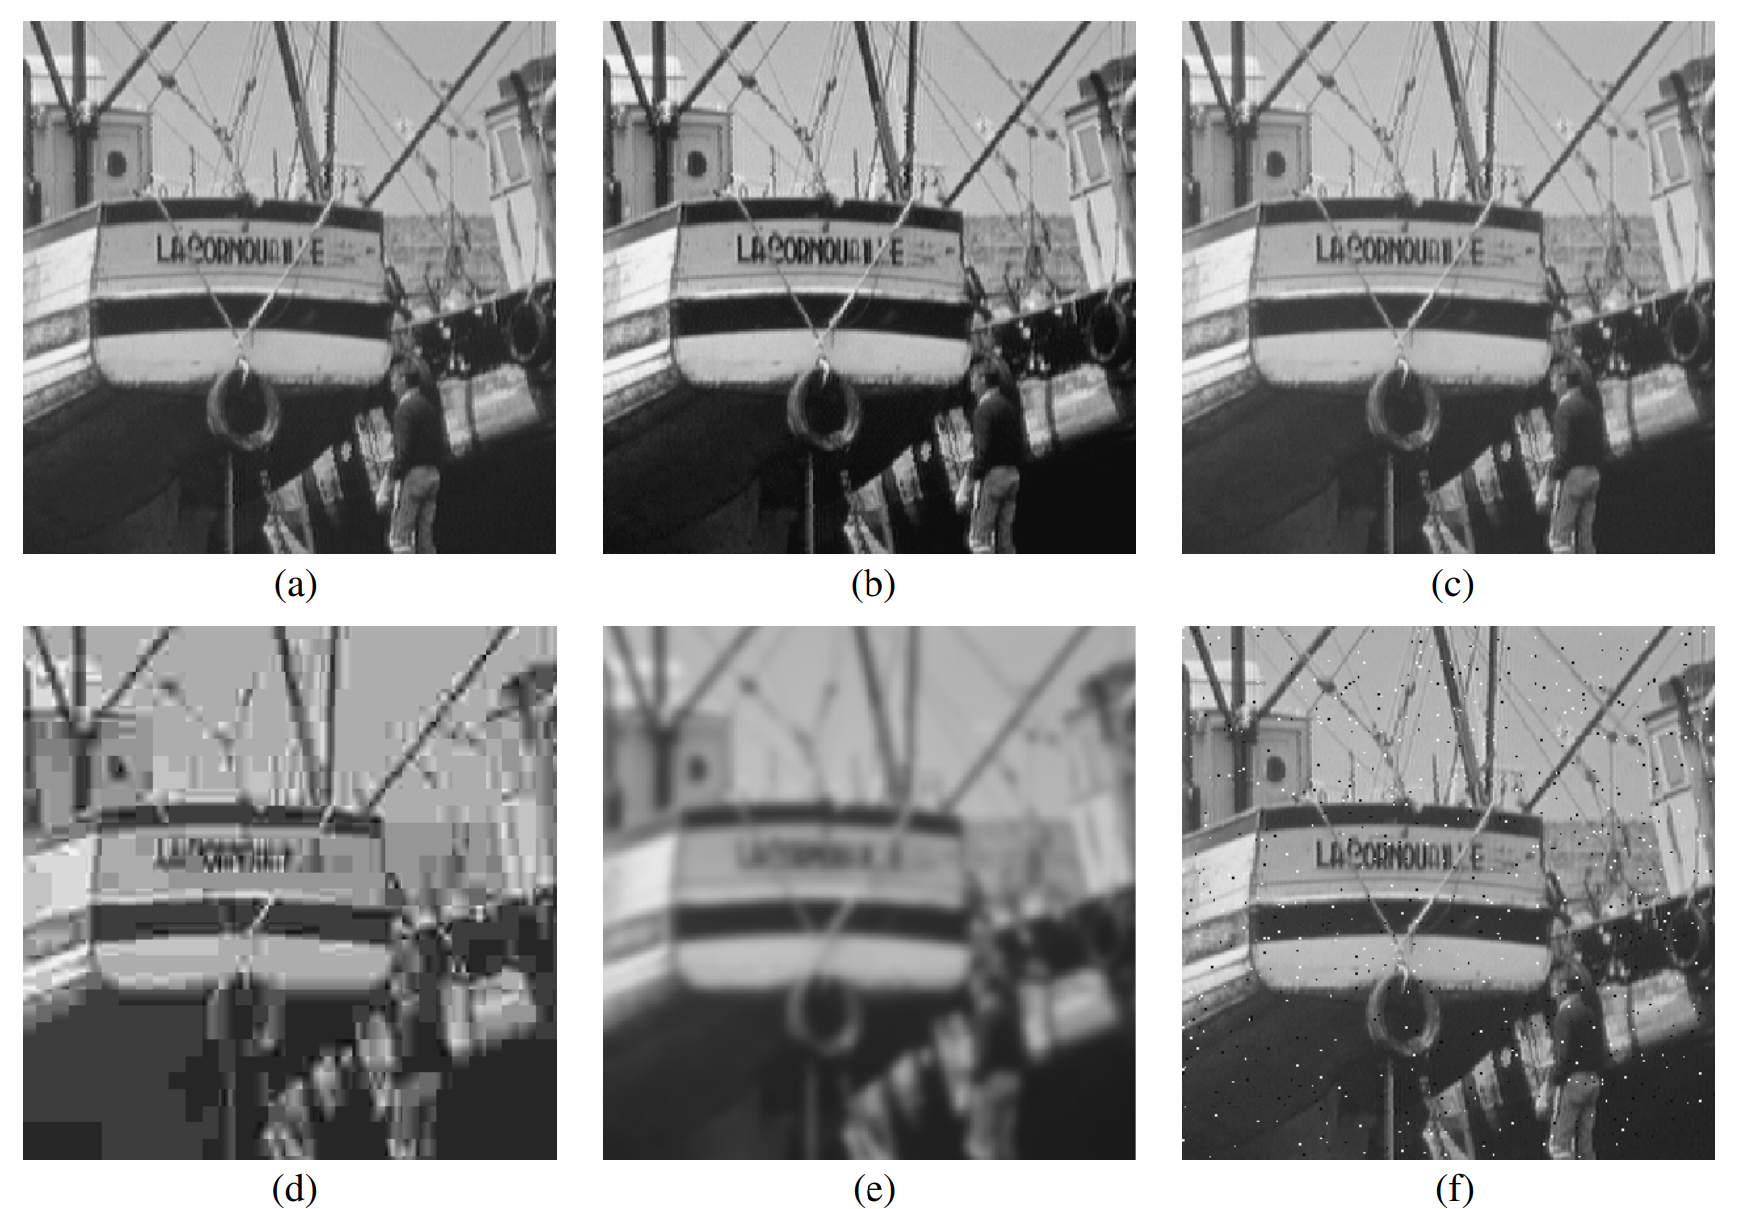
\includegraphics[width=0.90\linewidth,origin=c]{Report/Pictures/LossFuntion/MSE_SSIM_comparison.png}
    \caption{Different reconstructions all with MSE of 210}
    \label{SSIM MSE comparison}
\end{figure}


There have been many attempts at crafting a loss function that aligns better with the HVS. Two of the most notable examples are the SSIM\cite{SSIM} and the MS-SSIM\cite{MSSSIM}\cite{benchmark} that have been sited 43.529 and 5783 times respectively according to Google Scholar. The definitions are:
\begin{center}
    $l = \frac{2\mu_x\mu_y+c_1}{\mu_x^2+\mu_y^2+c1}$ \\
    $c = \frac{2\sigma_x\sigma_y+c_2}{\sigma_x^2 + \sigma_y^2 + c_2}$\\
    $s = \frac{\sigma_{xy} + c_3}{\sigma_x\sigma_y + c_3}$\\
    $SSIM = l^\alpha \cdot c^{\beta} \cdot s^\gamma $\\
    $MS\_SSIM = l_M ^ {\alpha_M} \cdot \prod_{j=1}^M c_j^{\beta_j} s_j^{\gamma_j}$
\end{center}

All these values are calculated on an 11x11 blocks of the image, these are then averaged for the total loss, sometimes called MSSIM and MMS-SSIM where the leading M stands for mean\cite{SSIM}\cite{MSSSIM}.
The MS-SSIM is based on the SSIM and they are quite similar and suffer from many of the same problems. We will mostly discuss the SSIM, since it is the most prevalent and the base of other loss functions like MS-SSIM, but most points discussed should be applicable for both loss functions\cite{ssimbad}\cite{MSSSIM}. The SSIM loss function is created under the assumption that the HVS is highly adapted for extracting structural information from a scene\cite{SSIM}. It then tries to exploit this by being a measure of structural similarity (hence the name Structural Similarity Index Measure). It is somewhat unclear whether or not the SSIM really measures structural similarity\cite{ssimbad}, but it does seam to align better with the HVS compared to the MSE. Looking back at figure \ref{SSIM MSE comparison}, the SSIM loss of images b to f are 0.9168, 0.9900, 0.6949, 0.7052, 0.7748, which aligns much better to our opinion compared to the MSE.

We did a small preprojekt on the subject (apendix A and B), where we used and compared the SSIM, MS-SSIM, MSE and the MAE (mean absolute error) loss functions. The SSIM and the MS-SSIM performed better visually, however, they were also less stable often suddenly blowing up or getting stuck. It was somewhat possible to circumvent these problems by reducing the learning rate and pretraining the network with more stable loss functions like the MAE or MSE. We also thought that the basis for the SSIM was too simplistic, since it is originally created for black and white images\cite{SSIM}\cite{MSSSIM}.

All these factores made it clear for us that we were not satisfied with the SSIM loss function. In our preproject (apendix A and B), we tried to improve upon the SSIM loss function, by splitting the image into its Ycbcr components and using the SSIM only for the Y component and other loss functions like the MAE on the chromatic components. The idea was that since the SSIM does not perform that well with color, and that the Y component should contain all the structural data, one could try to exploit the supposed strong sides of the SSIM while mitigating the weak aspects. This approach worked quite well, clearly outperforming the normal SSIM loss function after tweaking the resulting hyper parameters that arise from balancing the weight of the SSIM and the MAE loss functions. 

MÅSKE INDSÆTTE FIGUR FRA APENDIX A OG B HER???????????

However, we were still not satisfied with the results, we did not like that the SSIM is blocking the image in 11x11 squares, since this is one of the criticisms of the JPEG algorithm because it leads to blocking effects\cite{benchmark}\cite{JPEG}\cite{JPEG1.02}. We could also not find any good loss function to pair the SSIM with, since we could not find any loss function that aligns well with how the HVS perceive color. Furthermore, all the issues with the loss function being unstable were still present.

Furthermore \cite{ssimbad} shows that there are many other fundamental problems with the SSIM loss function, some of these are: There seams to be a direct relationship between MSE and SSIM, and since the MSE is not a perception-based metric, SSIM might not be one either\cite{ssimbad}. One can also derive the PSNR (Peak signal to noise ratio) from the SSIM which also sugests that SSIM is not a perception based index\cite{ssimbad}. There are also many weird cases where SSIM does not align well with the HVS \cite{ssimbad}, one is shown in the figure below:% der er andre kilder inde i ssimbad, som vi kan bruge i stedet for ssimbad over det hele.
\begin{figure}[H]
    \centering
    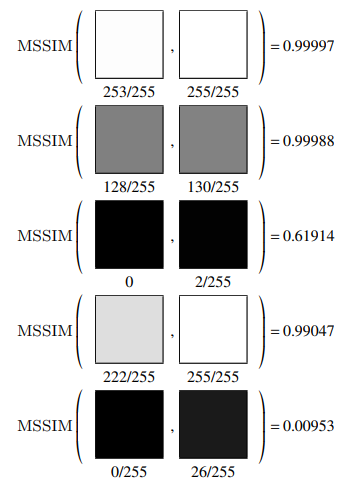
\includegraphics[width=0.40\linewidth,origin=c]{Report/Pictures/LossFuntion/SSIMBad.png}
    \caption{Misalignment with HVS and SSIM from\cite{ssimbad}}
    \label{Misalignment HVS SSIM}
\end{figure}

Where human judgement clearly disagrees heavily with the SSIM. Further they also show how poorly the SSIM can perform with color, and how large an influence the pixel density of the image has on the SSIM\cite{ssimbad}:
\begin{figure}[H]
    \centering
    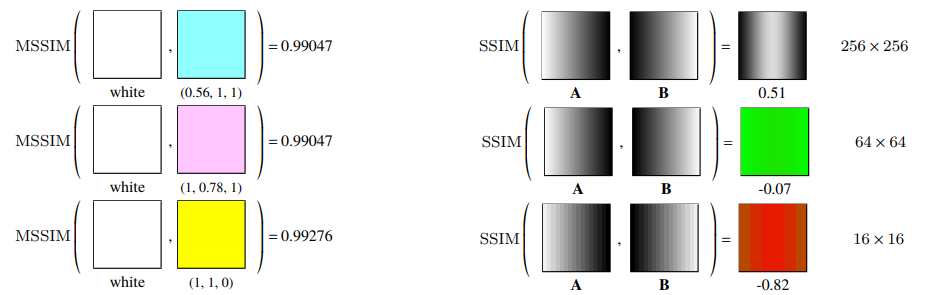
\includegraphics[width=0.90\linewidth,origin=c]{Report/Pictures/LossFuntion/color_and_cuality_comparison.png}
    \caption{Poor performance of SSIM caused by color and quality of images from\cite{ssimbad}}
    \label{Misalignment HVS SSIM color quality}
\end{figure}

Because of these problems, we will try to find a new loss function that aligns better with the HVS and has fewer problems than the SSIM.


\subsection{Our approach}
In order to find inspiration that might help us find or create a loss function superior to the above mentioned approaches, we look to related areas of research. 
Face recognition and face verification are two fields where hand crafted metrics and methods used to bee a weak link (We will refer to face recognition and face verification interchangeably, since both are applicable to our problem in the same way). \cite{benchmark}\cite{Learning_Fine_grained}\cite{Learning_similarity_metric}\cite{state_of_the_art}. The best face recognition pipelines used to rely on hand-engineered features\cite{state_of_the_art}, but the best modern approaches have discarded all hand crafted metrics, in favour of learned metrics\cite{state_of_the_art}\cite{UltimateAccuracy}\cite{FaceNet}\cite{Deep_Face}. 

When training a model to measure similarity between faces, one typically has a data set with multiple pictures of multiple people. One example being in \cite{Deep_Face} where they had 4.000.000 facial images belonging to more than 4.000 identities. There are a few different architectures that are most common for learning facial similarity, probably the most successful being the Siamese network with a triplet loss function\cite{Deep_Face}\cite{UltimateAccuracy}\cite{FaceNet}. A figure from \cite{Learning_Fine_grained} showing the architecture can be seen below:
\begin{figure}[H]
    \centering
    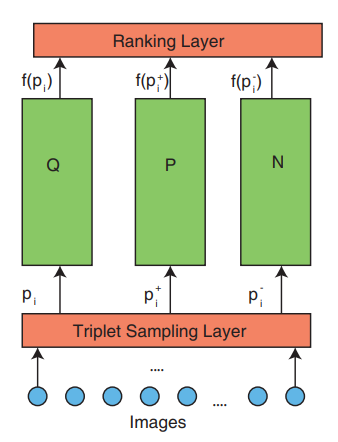
\includegraphics[width=0.50\linewidth,origin=c]{Report/Pictures/LossFuntion/Siamese.png}
    \caption{Siamese triplet loss architecture from\cite{Learning_Fine_grained}}
    \label{Siamese}
\end{figure}
Where Q, P and N are typically the same convolutional neural network (CNN) with identical parameters, and $P_i$ is the original image $P_i^+$ is the positive image (Different image of the same person), and $P_i^-$ is the negative image (Image of some other person)\cite{FaceNet}\cite{Learning_Fine_grained}. Where the triplet loss function defined by is:
\begin{center}
    $L = \sum_i^N[||f(P_i)-f(P_i^+)||_2^2-||f(P_i)-f(P_i^-)||_2^2+\alpha]_+$
\end{center}
Where f is the neural network representing Q, P and N. Due to the $\alpha$, the loss function forces $P_i$ and $P_i^+$ to be closer together than $P_i$ and $P_i^-$ as measured by the euclidean distance\cite{FaceNet}\cite{Learning_Fine_grained}. 
It is crucial for fast convergence, that $P_i^-$ is quite similar to $P_i$ and $P_i^+$, otherwise the task will be to easy for the network, and gradient descent will slow down to a crawl\cite{FaceNet}.

By using this approach, it was possible to discard all the hand-crafted metrics and get superior performance compared to methods that used hand crafted metrics\cite{state_of_the_art}\cite{UltimateAccuracy}\cite{FaceNet}\cite{Deep_Face}.

One could question the need of this rather complex architechture that outputs a point, rather than a more simple architechture that directly outputs if two faces match. One of the reasons why this architecture is so attractive for face recognition, is because the large computational load of neural networks, lead to it being beneficial to minimize the amount of images processed trough the network. By placing all images into a D dimensional space, one can efficiently compare N faces to one another, by only inserting each face into the model once, and using normal distance measures to compare outputs of the N different faces\cite{FaceNet}. This can reduce the parses trough the network from $O(N^2)$ to $O(N)$ when trying to find the two most similar faces in a database. This architecture also allows for paralellisation, since one can parse any number of images trough any number of neural networks and compare them afterwards. Further more, this method also allows for precomputation of all faces in a data set, such that if one wants to see if a new image has a match in the data set, one only needs to parse this one new image once trough the model, in order to compare it to all other images in the data set\cite{FaceNet}\cite{Learning_Fine_grained}\cite{Learning_similarity_metric}. Since typical face verification tasks, can contain a database of thousands of faces, efficiency and precomputation can be very important for a face verification tool.

Because of the complexity of the HVS and the lack of understanding about the HVS\cite{msebad}, we think that deep learning approaches might be even more needed in measuring human aligned image similarity, compared to face recognition. We think that this method should work for image similarity as well, because the tasks are very similar. However, we do not think that the computational advantages of this approach are going to have a large benefit for our needs. We will only use the distance metric as a loss function and will most likely not need to compare one image to more than one other image. 
Thus a simpler architecture that utilize the same ideas might be better for our needs, since it would make intuitive seance that a simpler approach would work better with a smaller data set and a smaller model. Furthermore a smaller network would also be faster, which in turn would speed up the training of the network that is supposed to use this loss function. These advantages would be great since we have limited computational resources.  Therefor we are going to try a simpler architecture, where we just merge the two images together into one image with 6 channels, and send it trough a simple CNN ending with some fully connected layers leading to one sigmoid activation function. 

MÅSKE LAVE EN FIGUR DER FORKLARER DET :):):):)

Other than the computational advantage, this architecture also allows us to have more control over the output of the loss function, since we can specify how large the loss between two images should be. Thus we do not need to group the images into a binary of acceptable and not acceptable (like $P_i^+$ and $P_i^-$), instead we can specify a continuous range of acceptability depending on how similar the images are.


With an idea of the architecture in mind, we still need a data set of different images and their reconstructions. As briefly discussed in the section about our data, we do not know any such data set with images graded by humans for their similarity. Furthermore, it does not even seam possible to get a data set of all possible reconstructions of an image. 

Since lossy image reconstructions are in a way an image augmentation, we try to tackle the problem of lacking data, by implementing image augmenting functions, that can augment images in different ways to varying degrees of human acceptability.
By having more augmenting functions, we can specify more clearly to the neural network what kind of augmentations are acceptable and which are not. The hope is that the neural network can use this information to gain more axis of freedom, allowing it to compress the image into a smaller space. We ended up implementing XXXXXXXXXX augmenting functions, some examples of images being transformed by the functions can be seen below:

\begin{figure}[H]
    \centering
    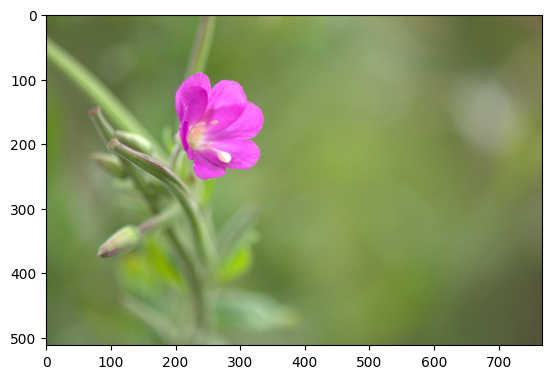
\includegraphics[width=0.80\linewidth,origin=c]{Report/Pictures/LossFuntion/Original.png}
    \caption{Original}
    \label{Original}
\end{figure}

\begin{figure}[H]
    \centering
    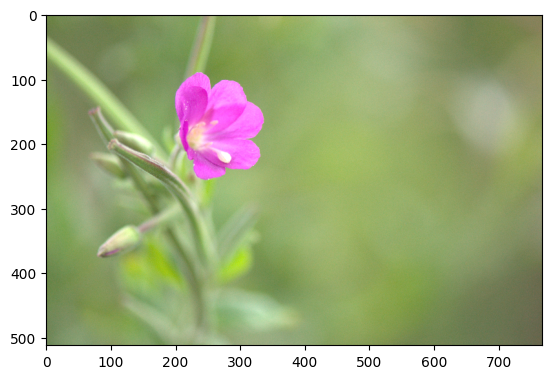
\includegraphics[width=0.45\linewidth,origin=c]{Report/Pictures/LossFuntion/Add20.png}
    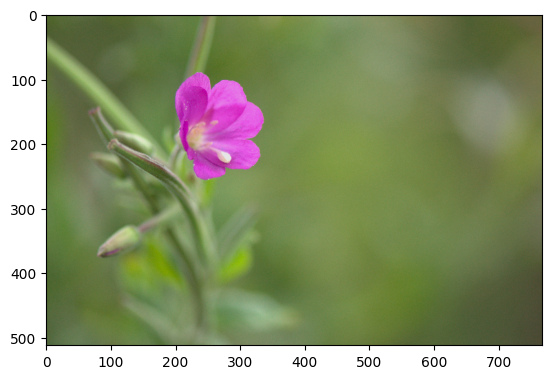
\includegraphics[width=0.45\linewidth,origin=c]{Report/Pictures/LossFuntion/Mul0_9.png}
    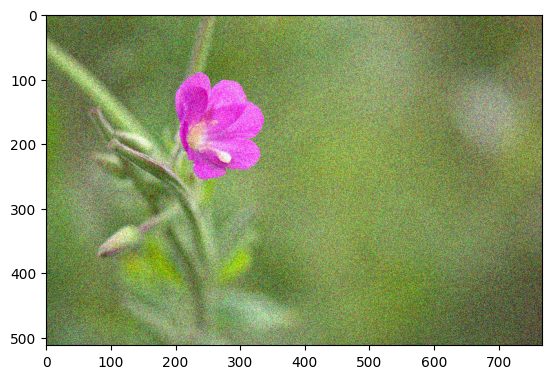
\includegraphics[width=0.45\linewidth,origin=c]{Report/Pictures/LossFuntion/UniformNoise.png}
    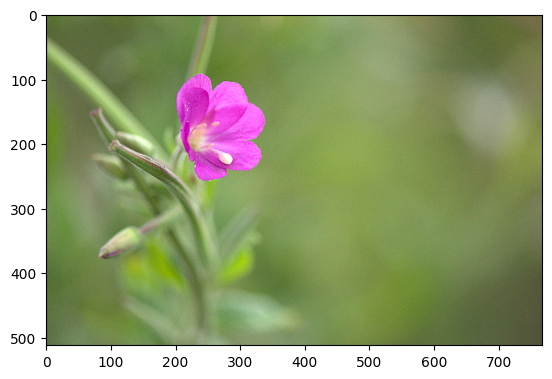
\includegraphics[width=0.45\linewidth,origin=c]{Report/Pictures/LossFuntion/UnsharpMasken.png}
    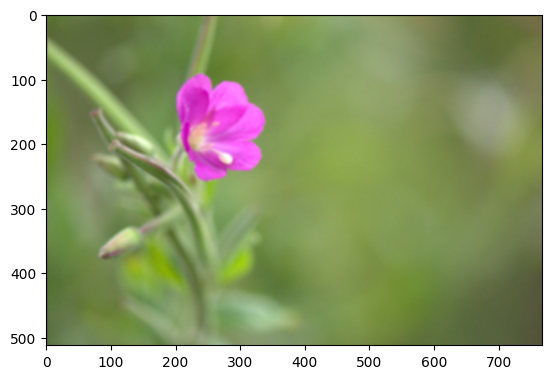
\includegraphics[width=0.45\linewidth,origin=c]{Report/Pictures/LossFuntion/BoxBlur5x5.png}
    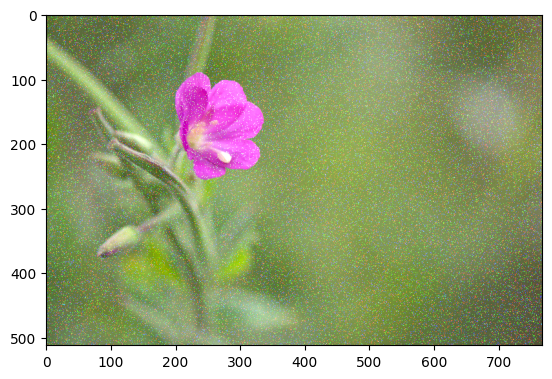
\includegraphics[width=0.45\linewidth,origin=c]{Report/Pictures/LossFuntion/Salt.png}
    \caption{From top left: Adding to all pixels, multiplying constant on all pixels, adding uniform noise, unsharp masking, Box blur, salting}
    \label{distortions}
\end{figure}

The functions we implemented came in a few different types: different Kernels, different types of random noise, adding or multiplying all pixels by values, JPEG with more. All of these can apply various degrees of distortion to an image, making our data set explode in size. Since the image data set is so large, while our computational resources are limited, efficiency is important. Most of our code makes use of optimized code from libraries, but to apply different kernels to the image, we make use of Fast Fourier Transform to greatly improved the running time. In total we reviewed 75 different settings of different functions, giving us a data set 75 times larger than before, containing image pairs with a similarity score. These similarity scores range from 0 being no noticeable difference, to 1 being a large difference. 

HVIS VI HAR FLYTTET NOGET AF DET TIL RUST SKAL DET NOK SKRIVES HER!!!!!!!


This seams to work quite well, but there are some disadvantages compared to if the images themselves where graded. One excample can be seen in the figure below:
SFGYHUFJISHVYIEDKUXCNALHFNAOILHFNVAS

Where it is clear that the transformation does not have the same effect on both images, as judged by the HVS. 